\documentclass{article}

\usepackage[utf8]{inputenc}
\usepackage[ngerman]{babel}
\usepackage{amsmath}
\usepackage{url}
\usepackage[pdftex]{graphicx}
\usepackage{listings}
 
\setcounter{secnumdepth}{6}
\title{Object Caching\\Project Proposal}
\author{Lukas Hofmaier, Raphael Kohler, Timon Brüllmann}
\date{\today}
\begin{document}
\maketitle
\vspace{1cm}
\section{Betreuer}
J.M.Joller  Abteilung für Informatik HSR/FHO

\section{Motivation}
Mercury ist ein Datenverarbeitungssystem, welches es Clients ermöglicht, Methoden von Objekten über das Netzwerk aufzurufen. Dabei entstehen unter anderem folgende zwei Problembereiche, auf welche das Augenmerk dieser Studienarbeit gelegt wird:

\begin{itemize}
\item Clients können Werte von Instanzvariablen von Objekten auf dem Server lesen. Die Clients können diese Werte im Hauptspeicher abspeichern und zu einem späteren Zeitpunkt in einer kausal abhängigen Methode als Argument einsetzen. Dabei kann ein Lost Update auftreten.
\item Alle Methodenaufrufe werden über das Netzwerk an den Server gesendet. Die Methodenaufrufe auf den Clients sollen schneller werden.
\end{itemize}

\section{Ziele der Arbeit}
Die Arbeit wurde durch Mercury motiviert, unserer Ziele sind jedoch losgelöst von diesem System, da die genannten Probleme bei allen verteilten Software-Systemen auftreten.

\subsection{Prioritäten}
\label{sec:prioritaeten}

\begin{enumerate}
\item Das ‘‘Lost Update’’-Problem soll vermieden werden:
\begin{itemize}
\item Instanzvariablen eines Objekts können durch mehrere Clients
  modifiziert werden. Liest ein Client den Wert eines Datenfeldes und
  verwendet er diesen Wert später als Argument in einer kausal
  abhängigen Schreibmethode, so muss sichergestellt werden, dass der Wert
  zwischen der Lese- und der Schreiboperation nicht von einem anderen
  Client verändert wurde. Wird dies nicht sichergestellt, kann es dazu führen, dass Änderungen, welche ein anderer Client zwischenzeitlich gemacht hat, verloren gehen.
\end{itemize}
\item Die Abhandlung der Schreib -und Lesezugriffe auf das Objekt, welches auf dem Server liegt, soll für den Client möglichst schnell passieren.
\end{enumerate}

\subsection{Hauptziele}
\label{sec:hauptziele}

\subsubsection{RMI mit Concurrency Control}
\label{sec:rmi-mit-concurrency}

In dieser Semesterarbeit soll ein Konzept erarbeitet werden, welches Lost Updates bei kausal abhängigen Methoden verhindert.  Zudem soll ein vereinfachtes RMI System implementiert werden, welches zeigen soll, ob sich dieses Konzept einfach realisieren lässt.

\subsubsection{Testframework}
\label{sec:testframework}

Um das System zu testen, wird parallel dazu ein Testframework entwickelt. Dieses Framework soll in der Lage sein, unterschiedliche RMI Systeme als Server und Clients zu starten. Das Testframework ist in der Lage, eine Szenariobeschreibung einzulesen und dieses Szenario mit dem zu testenden System durchzuspielen. Ein Szenario lässt sich leicht spezifizieren und besteht aus einer Abfolge von Methoden-Aufrufen, welche der jeweilige Client tätigen muss. Das Framework sammelt dabei Messdaten über die Zeitdauer der einzelnen Methodenaufrufe. Die Messdaten sollen es ermöglichen abzuwägen, welche Systeme mit welchen Parameter sich für welchen Anwendungszweck eignen. Das Testframework registriert das Auftreten von Schreib-Konfikten beim Aufruf von Schreibmethoden. Alle Messdaten werden in Dateien gespeichert, was eine spätere Interpretation der Resultate ermöglicht.

\subsection{Erweiterte Ziele}
\label{sec:erweiterte-ziele}

\subsubsection{Object Caching}
\label{sec:object-caching}

Um die Dauer von Methodenaufrufen zu verkürzen, soll das RMI System um
einen Object Cache erweitert werden. Methoden ohne Seiteneffekte
werden auf den Objekten im Cache ausgeführt. Für das System wird ein
passendes Konsistenzmodell ausgewählt. Das Konsistenzmodell
Einschränkungen für Leseoperationen. Es definiert Regeln, die
definieren, wie aktuell Werte sind, die bei einer Leseoperation
zurückgegeben werden. Dieses Modell wird durch ein geeignetes Konsistenzprotokoll durchgesetzt. Der User muss die Methoden eines Objekt markieren, damit das System zwischen Methoden mit Seiteneffekt und solchen ohne Seiteneffekt unterscheiden kann. Methoden die Seiteneffekte aufweisen, werden auf dem Server ausgeführt, die Restlichen können direkt auf dem lokal zwischengespeicherten Objekt ausgeführt werden.

\subsubsection{Entwicklung neuer Szenarien}
\label{sec:entwicklung-neuer-szenarien}

Um die Lösungen mit und ohne Cache miteinander vergleichen zu können,
müssen neue Testszenarien geschrieben werden können. Neue
Testszenarien können über eine XML-Beschreibung spezifiziert werden.

\subsubsection{Feingranulares Locking}
\label{sec:feingr-lock}

Der Concurrency-Mechanismus soll es ermöglichen, dass Anfragen parallel ausgeführt werden können.

\subsection{Szenario}
\label{sec:szenario}

Als Ausgangslage für das gesamte Projekt wird folgendes Szenario eingesetzt:

\subsubsection{Deployement}
\label{sec:deployement}

Es wird ein verteiltes System mit einem Server und zwei Clients verwendet.
\begin{center}
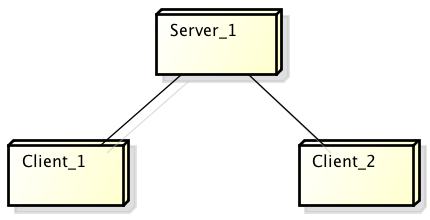
\includegraphics[scale=0.85]{Deployment.png}
\end{center}

\subsubsection{Kausaler Zusammenhang}
\label{sec:kaus-zusamm}

Die Clients möchten den Kontostand um 10 \% erhöhen. Dazu führen die Clients folgende Schritte aus:
\begin{lstlisting}
1. b = getBalance();
2. setBalance( b * 1.1 );
\end{lstlisting}

\noindent Diese Schritte werden zum Prozess ‘‘Kontostand Erhöhen’’ zusammengefasst.

\subsubsection{Account Typ}
\label{sec:account-typ}

Auf einem Server wird ein Account-Objekt instanziert Die
Zugriffssynchronisation wird nicht über den in Java eingebauten
Mechanismus synchronized direkt auf den Methoden realisiert. Das RMI
System ist für die Zugriffssynchronisation verantwortlich. Das Interface von Account sieht wie folgt aus:
\begin{lstlisting}
public interface Account {
    public int getBalance();
    public void setBalance(int balance);    
}
\end{lstlisting}
Zwischen getBalance und setBalance besteht ein kausaler Zusammenhang: setBalance darf nur ausgeführt werden, wenn das Argument balance aktuell ist. Ist der Wert nicht mehr aktuell, wird der ‘‘Kontostand-Erhöhen’’-Prozess abgebrochen. Der Client wiederholt in diesem Fall den gesamten Prozess (aktuelle Daten holen, Daten schreiben) automatisch.

Dem Client ist das Interface Account bekannt. Das Interface wird vor Prozessstart deployed.
Zwei Clients beschaffen sich eine Referenz, in Form eines
Proxy-Objektes, auf das Account-Objekt. Das Proxy-Objekt leitet
Methodenaufrufe des Clients an den Server weiter und nimmt
Rückgabewerte vom Server entgegen. Der entfernte Methodenaufruf ist
für den Client transparent.

\subsubsection{TestFramework}
\label{sec:testframework-1}


Bei jedem Szenario werden folgende Messdaten festgehalten.
\begin{itemize}
\item durchschnittliche Dauer des Methodenaufrufs getBalance()
\item durchschnittliche Dauer des Methodenaufrufs setBalance()
\item Anzahl aufgetretene Konflikte
\item Dauer eines setBalance(); Methodenaufrufs im Falle einer Konfliktsituation
  \begin{itemize}
  \item Zeitdifferenz zwischen erstem setBalance bis erfolgreichem setBalance
  \item Zeitdifferenz zwischen setBalance und Empfang der zugehörigen Exception
  \end{itemize}
\end{itemize}

\subsubsection{Test-Szenarien}
\label{sec:test-szenarien}

\paragraph{Konfliktloser Zugriff}
\label{sec:konfl-zugr}
$~~$ \\
Das Szenario soll zeigen, wie lange Methodenaufrufe dauern, wenn keine Konflikte auftreten. Ein Client führt den Prozess Kontostand-Erhöhen 10000-mal aus.

\paragraph{Race Condition}
\label{sec:race-condition}
$~~$ \\
Das Szenario soll zeigen wie viele Konflikte auftreten, wenn beide Clients permanent Kontoerhöhungen ausführen wollen.
Beide Clients führen den Prozess Kontostand-Erhöhen 10000 mal aus. Der Server startet die Clients, mit einer möglichst kleinen Verzögerung, hintereinander. 

\paragraph{Erzwungene Konflikte}
\label{sec:erzwungene-konflikte}
$~~$ \\
In diesem Szenario soll jeder setBalance-Aufruf von Client2 zu einer Konfliktsituation führen. Damit sind Konfliktsituation nicht dem Zufall überlassen, sondern treten zuverlässig auf und können besser analysiert werden.

\noindent Dies wird folgendermassen erreicht:
\begin{itemize}
\item Client1 führt ununterbrochen Kontoerhöhungen aus
\item Client2 führt 100 Kontoerhöhungen aus. Nach dem getBalance()-Aufruf wartet Client2 10ms
\item Währenddessen führt Client1 eine Schreiboperation aus
\item Dadurch werden die Daten im Speicher von Client2 veraltet
\item Client2 führt nun eine Schreiboperation aus und erhält eine Konfliktmeldung
\end{itemize}

\section{Sitzungen}
Mit dem Betreuer dieser Arbeit findet eine wöchentliche Sitzung statt. Dabei werden die Fortschritte besprochen und falls vorhanden, offene Fragen diskutiert. Die Länge der Sitzung ist daher variabel, je nachdem ob und wieviele offene Fragen und Probleme bestehen. Die Entscheidungen, sowie die diskutierten Punkte, werden in einem Sitzungsprotokoll schriftlich festgehalten.


\vspace{2cm}

\noindent Rapperswil, den \date{\today} \\
\end{document}
